\documentclass{standalone}
\begin{document}
	\chapter{Lung Lesion Segmentation}
	

	The aim of this works of thesis is to develop a pipeline for identification of GGO and CS areas in chest CT scans of patients affected by COVID-19, with following characteristics:   
	\begin{itemize}
		\item  \textbf{Fully Automated: } to remove the dependency from any external operator, and so the subjectivity to its experience. 
		
		\item \textbf{Fast: } in order to compete with certified software and to provides a segmentation in few minutes.
	\end{itemize}
	
	Before start to speak about the the pipeline, is useful to define the areas we wish to identify.
	
	Austin in ~\cite{ART:Austin} has defined the GGO and CS as :  
	\begin{center}
	"\emph{Hazy increased attenuation of lung, but with preservation of bronchial and vascular margins; caused by partial filling of air spaces, interstitial thickening, partial collapse of alveoli,normal expiration, or increased capillary blood volume, which is different from consolidation in which bronchovascular margins are obscured.}
	\end{center}. 
		
	\begin{figure}[h!]
		\centering
		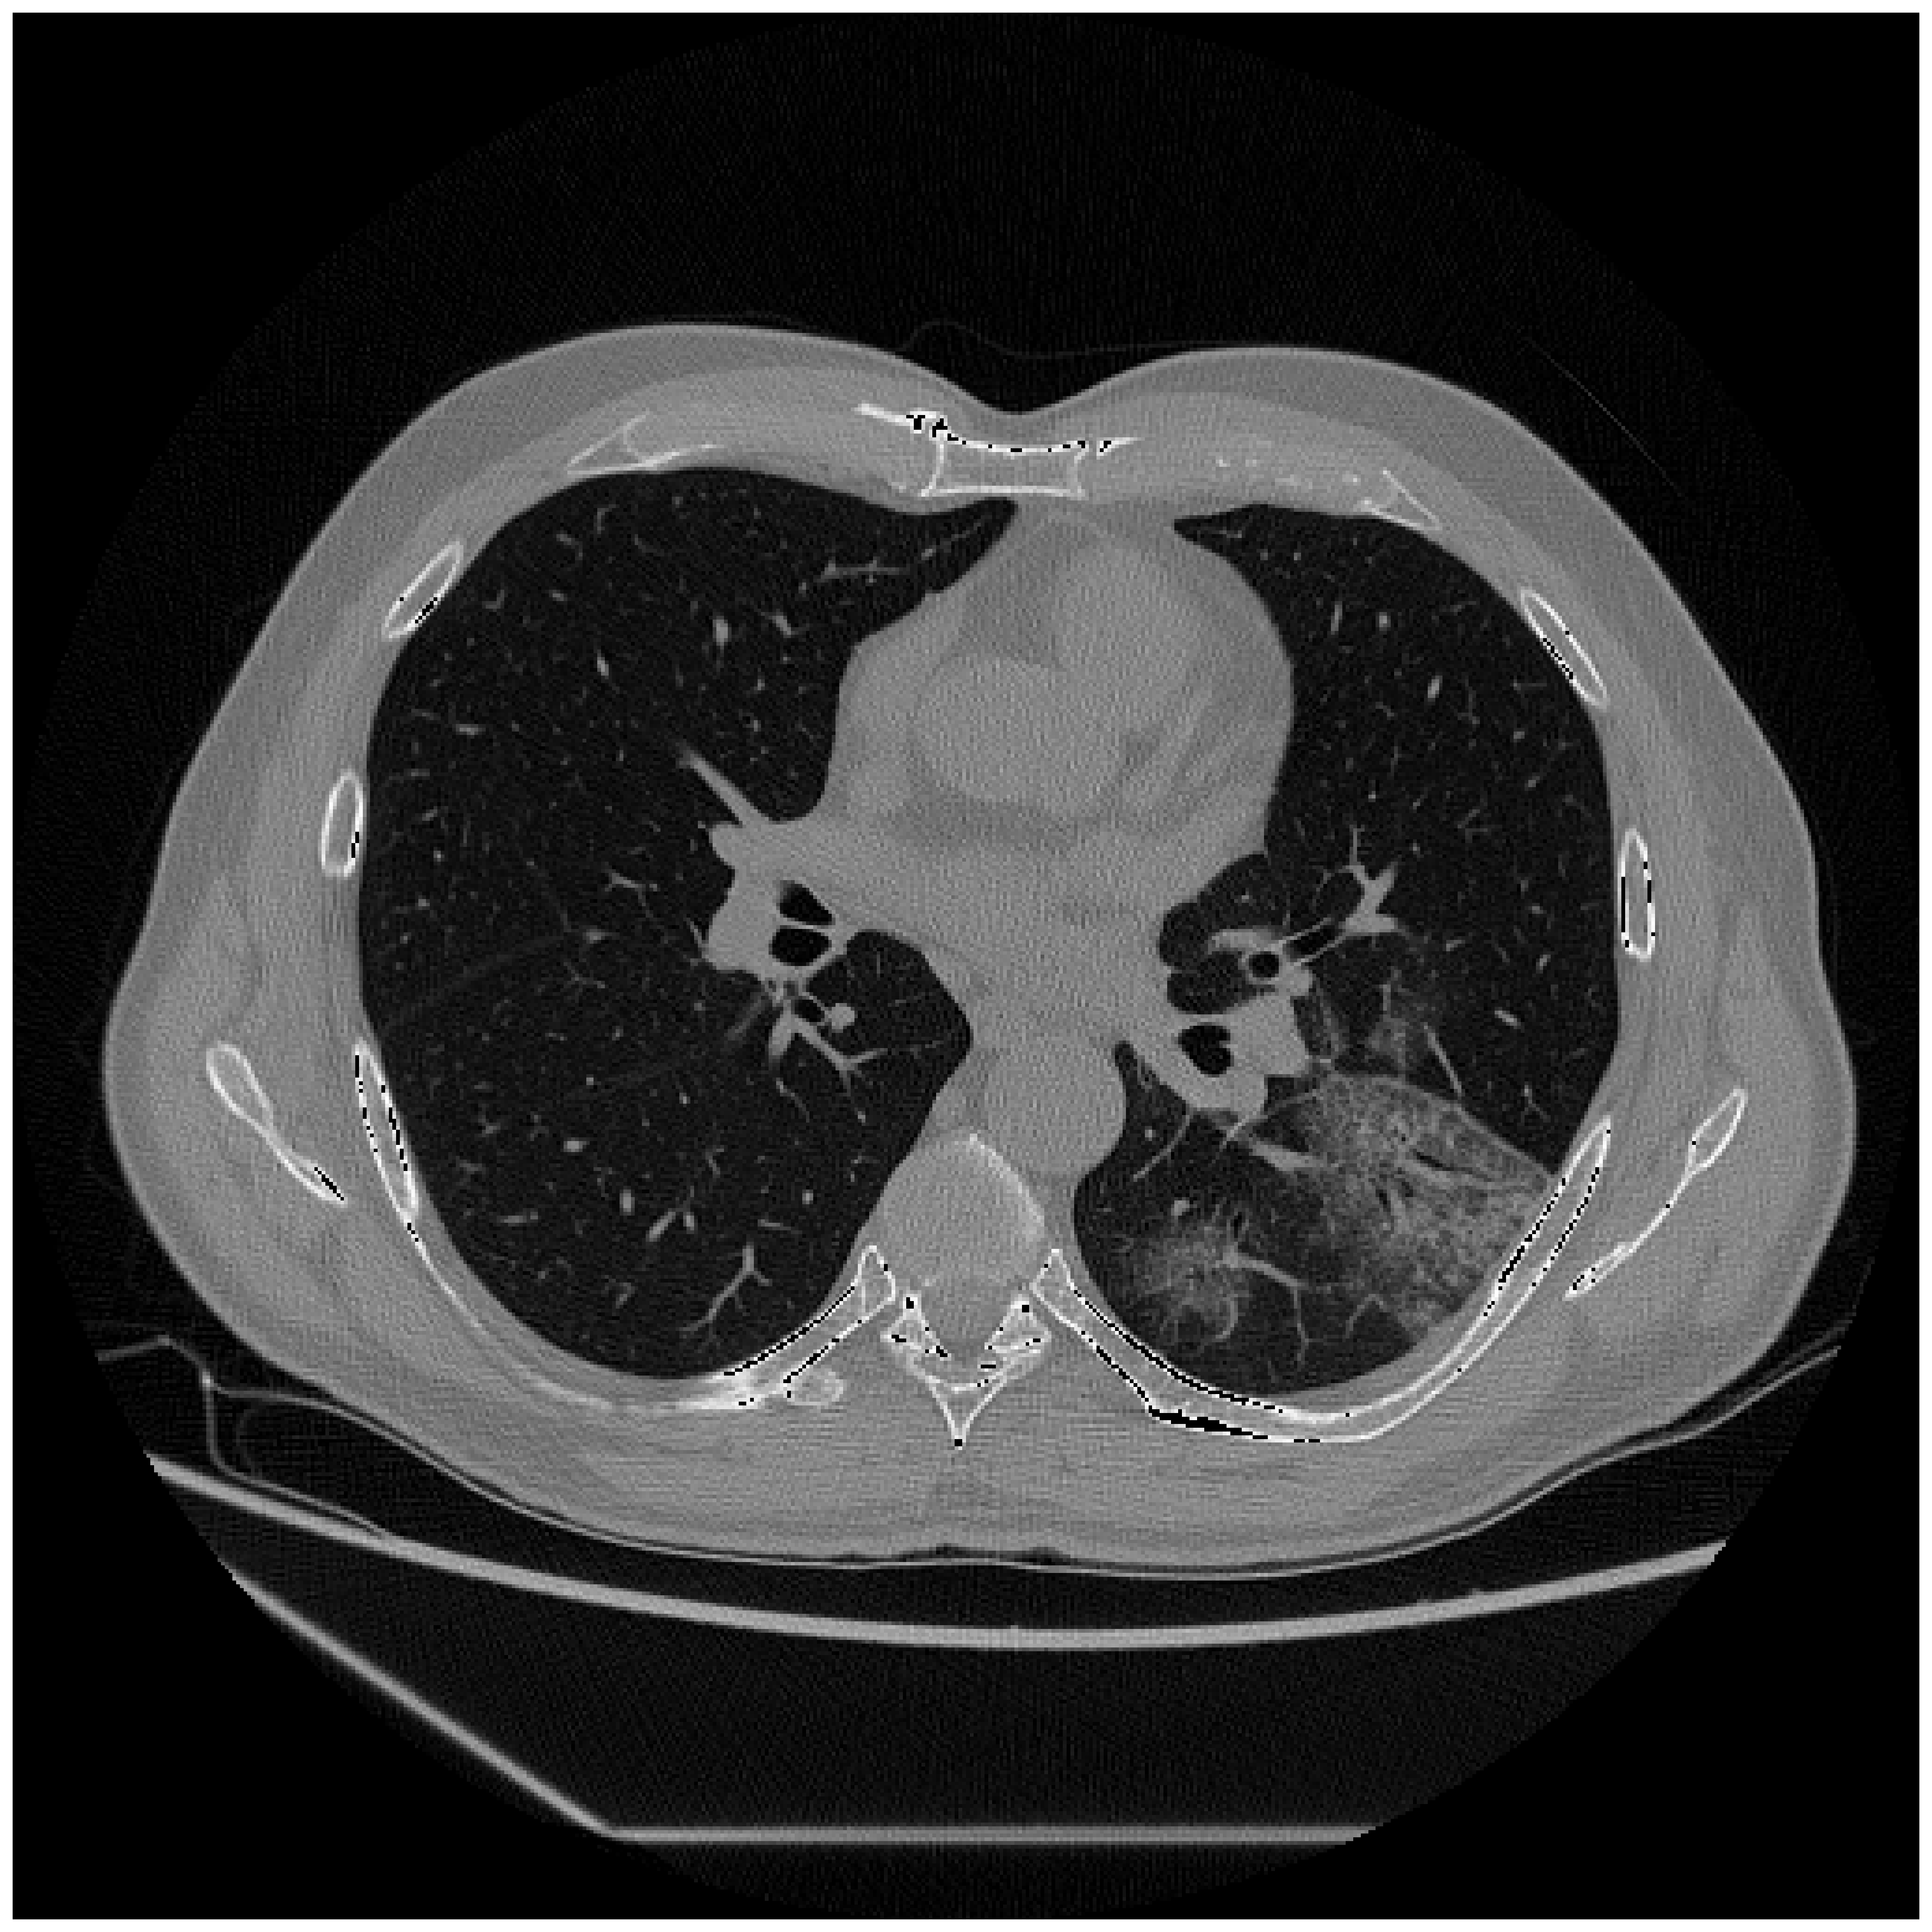
\includegraphics[scale=.5]{GGO.png}
		\caption{Chest CT image of a patient affected by COVID-19. We can see GGO and CS on the right lung. We can appreciate how the different structures, like lesions, are identified by similar color, so the basic segmentation idea was to group voxel by color similarity.}
		\label{fig:GGO}
	\end{figure}

	An example of these areas is in \figurename\,\ref{fig:GGO}, in which chest CT scan of patient affected by COVID-19 are visualized.
	We can notice that the different structures are characterized by similar gray level: the basic idea was to use the color quantization for medical image segmentation, grouping voxels based on color similarity, and  assigning  to each tissue a characteristic color. This can be done since in CT scan exists a relationship between the tissue in the voxels and the Gray Levels used to display it, given by the Hounsfiend Units(eq\,\ref{eq:HU}): the colors are proportional to HU, which are defined as a linear transformation of the linear attenuation coefficient($\mu$).
	
	We can consider different properties beside the single voxel intensity. As we can see, lesion areas involves many closest voxels. It is interesting to incorporates also neighborhood voxel information in the color quantization. Moreover, contrast between sick and healthy areas may change according to the severity of the disease. As a consequence it is interesting to incorporates also different gamma of the image, in order to enhance these regions.
	
	To takes into account these multiple information, I've build a multichannel image in which each channel corresponds to a different image property. To exploites these properties I've applied different filters to the raw image tensor. 
	
	In this way I've build a color space in which each primary color corresponds to a different image property.
		
	Once I've build the color space, we I've to find the characteristic color of each tissue under study, which is represented by a centroids in the color space. In order to perform this task and to achieve the centroids estimation, a simple k-means clustering was used, since it provides a good balance between segmentation performance and computational efficiency.
	
	K-means clustering requires a prior knowledge about the number of cluster, which in our case is given by the anatomical structure of the lung. I have consider a different cluster for each anatomical structure.
	Once I have estimated the centroids for each tissue, I have used them for the actual segmentation, by assign each voxel to the cluster of the closest centroids
			
	Before each of these steps we need a preliminary phase that aim to isolate the lung regions in order to exclude the extra lung areas and reduce false positives and motion artifacts.
	In the end the pipeline structure is divided in three main blocks as we can see in \figurename\,\ref{fig:Pipeline}. Each block will perform a different step of the segmentation: 
	\begin{itemize}
		\item \textbf{Pre-Processing and lung extraction}: Preliminary step, it involves the registration of HU, isolation of lung regions and removal of bronchial structures and motion artifacts.
		
		\item \textbf{Training}, that compute the set of centroids used for segmentation. It involves the clustering of a training dataset. 
		
		\item \textbf{Labeling} :  that assign each voxel to the cluster with the closest centroids.
	\end{itemize}
	
	
	\begin{figure}[h!]
		\centering 
		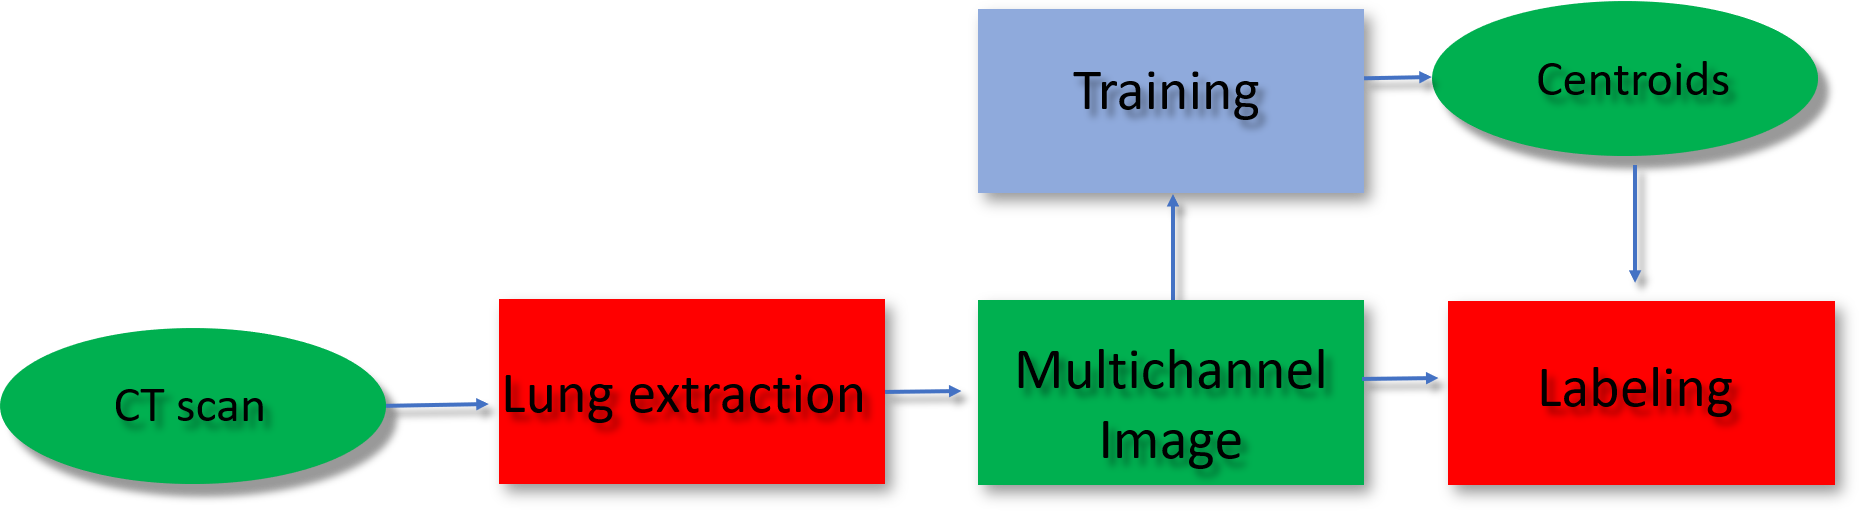
\includegraphics[scale=.6]{Pipeline.png}
		\caption{Flow chart of the main structure of the developed pipeline. The training process, which allows the estimation of the centroids, is performed only one time.}\label{fig:Pipeline}
	\end{figure} 
	
	
	The training step is the one which allows the estimation of the centroids. Once the centroids are estimated this step is no more necessary. 
	In the end the segmentation pipeline results in only two steps: \textbf{lung extraction} and \textbf{labeling}. The final structure is summarized in \figurename\,\ref{fig:FinalPipeline} in which we can observe the flowchart of each step with an image that shows the partial results.
	
	\begin{figure}
		\centering
		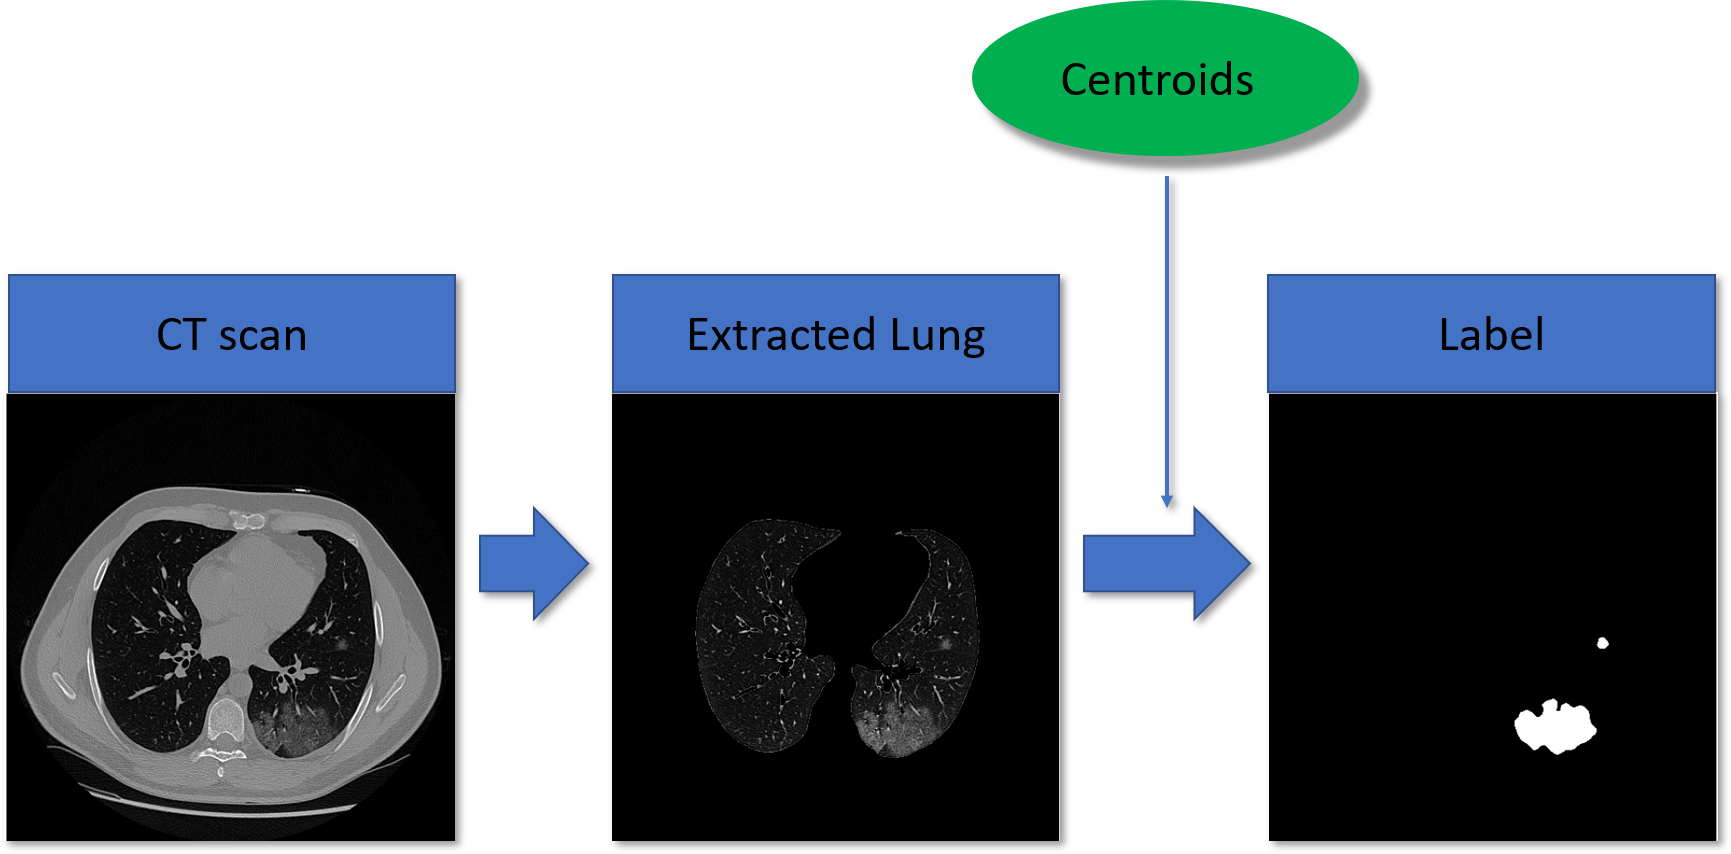
\includegraphics[width=.87\textwidth]{final_pipeline.png}
		\caption{Actual segmentation step, from left to right we can see the input image stack, the isolated lung regions and the final label. To performed the labeling a set of pre-computed centroids was used.}\label{fig:FinalPipeline}
	\end{figure}

\end{document}